% **************************************************************
% Feeding a Nation --- EcoMod2026 presentation
% Lehigh Beamer theme (visual style only; content is the MBG paper)
% **************************************************************

\documentclass[11pt,aspectratio=169]{beamer}
\usepackage{amsfonts,amsmath}
\usepackage{graphicx}
\usepackage[export]{adjustbox}
\usepackage{multicol}
\usepackage{setspace}
\usepackage{array}
\usepackage{pgfplots}
\pgfplotsset{compat=1.18}
\usepackage{booktabs}
\usepackage{colortbl}
\usepackage{tabularx}
\newcolumntype{C}{>{\centering\arraybackslash}X}
\usetikzlibrary{tikzmark,arrows.meta,positioning}

\usetheme{lehighlight}
\usefonttheme{serif}

\AtBeginSection[]{
  \begingroup
    \setbeamertemplate{footline}[sectionfootline]
    \setbeamertemplate{section page}[mysection]
    \frame[c]{\sectionpage}
  \endgroup
}

% ==================///==================///==================///
% ==================/// SPLASH PAGE
% ==================///==================///==================///

\title{Feeding a Nation}
\subtitle{\scriptsize\shortstack[r]{Regional Food Inflation, Welfare, and Trade Regimes\\ under Indonesia's Free Nutritious Meals Program}}
\author[A.\ A.\ Yusuf et al.]{\tiny Arief Anshory Yusuf, Khrisna Gupta, M.\ Firman Hidayat, Devy Pratiwi, Bambang Indra Ismaya}
\institute{\tiny Universitas Padjadjaran $\cdot$ Dewan Ekonomi Nasional $\cdot$ Bank Indonesia}
\date{\tiny EcoMod2026 $\cdot$ University of Luxembourg, Luxembourg $\cdot$ 8--10 July 2026}
\titlegraphic{
\includegraphics[width=1.25in]{Lehigh-Logo-PMS.png}}

% ==================///==================///==================///
% ==================/// START PRESENTATION
% ==================///==================///==================///

\begin{document}
\begin{frame}[t]
\titlepage
\end{frame}

% ==================///==================///==================///
% ==================/// BODY
% ==================///==================///==================///

\section{Motivation}

\begin{frame}{MBG at a Glance: A Fiscal Event, Not Just a Meal Program}
\centering
\begin{columns}[T,onlytextwidth]
	\column{0.23\textwidth}\centering
	\fcolorbox{lubrown}{lubrown10}{\begin{minipage}{0.9\linewidth}\centering\vspace{4pt}{\Large\textcolor{lubrown}{\textbf{USD 20B}}}\\[2pt]{\scriptsize 2026 budget}\vspace{4pt}\end{minipage}}
	\column{0.23\textwidth}\centering
	\fcolorbox{lubrown}{lubrown10}{\begin{minipage}{0.9\linewidth}\centering\vspace{4pt}{\Large\textcolor{lubrown}{\textbf{9\%}}}\\[2pt]{\scriptsize of state expenditure}\vspace{4pt}\end{minipage}}
	\column{0.23\textwidth}\centering
	\fcolorbox{lubrown}{lubrown10}{\begin{minipage}{0.9\linewidth}\centering\vspace{4pt}{\Large\textcolor{lubrown}{\textbf{83M}}}\\[2pt]{\scriptsize recipients}\vspace{4pt}\end{minipage}}
	\column{0.23\textwidth}\centering
	\fcolorbox{lubrown}{lubrown10}{\begin{minipage}{0.9\linewidth}\centering\vspace{4pt}{\Large\textcolor{lubrown}{\textbf{34}}}\\[2pt]{\scriptsize provinces}\vspace{4pt}\end{minipage}}
\end{columns}
\bigskip
\footnotesize
\begin{itemize}\setlength\itemsep{5pt}
	\item Indonesia's \textit{Makan Bergizi Gratis} (MBG): launched January 2025, flagship program of the Prabowo administration --- one of the largest single fiscal commitments in the national budget.
	\item Targets pregnant women, toddlers, and school children from primary through upper-secondary school.
\end{itemize}
\smallskip
{\tiny\textit{For context: total global school-feeding expenditure by domestic governments $\approx$ USD~48bn (2022, all countries combined). India's Midday Meal Scheme reaches $\approx$100M but covers only primary/lower-secondary. Brazil $\approx$40M since the 1950s. South Korea $\approx$7M. MBG's combination of universal provision, wide age coverage, and fiscal scale is without precedent globally.}}
\end{frame}

\begin{frame}{The Policy Tension: Feeding 83 Million amid a Legacy of Trade Protection}
\footnotesize
\begin{columns}[T,onlytextwidth]
	\column{0.54\textwidth}
	\begin{itemize}\setlength\itemsep{6pt}
		\item Five decades of Indonesian trade policy: persistent oscillation between liberalisation and protection.
		\item Protectionist tendencies reassert themselves under economic shocks, political transitions, and rising economic nationalism.
		\item Trade regime heavily reliant on non-tariff measures; food self-sufficiency is a politically entrenched, securitised narrative that survives economic evidence to the contrary.
		\item MBG's unprecedented food procurement --- poultry, eggs, vegetables, dairy, rice, and more, across 34 provinces --- collides directly with this self-sufficiency agenda.
	\end{itemize}
	\column{0.42\textwidth}
	\centering
	{\scriptsize\textcolor{lubrown}{\textbf{Effective rate of protection, 2015}}}\\
	{\tiny (price + quantitative restrictions; Marks, 2017)}
	\vspace{6pt}

	\begin{tabular}{lr}
		\toprule
		\textbf{Commodity} & \textbf{ERP (\%)} \\
		\midrule
		Rice       & 103.6 \\
		Sugar      &  87.6 \\
		Corn       &  27.9 \\
		Fruits     &  27.2 \\
		Vegetables &  21.8 \\
		Livestock  &  16.3 \\
		\bottomrule
	\end{tabular}
\end{columns}
\end{frame}

\section{Research Questions}

\begin{frame}{Three Research Objectives}
\footnotesize
\begin{enumerate}\setlength\itemsep{12pt}
	\item \textbf{Quantify} the economy-wide macroeconomic consequences of MBG --- on prices, sectoral output, and household welfare --- under three alternative policy scenarios: import protection, free trade, and productivity-led supply expansion.
	\item \textbf{Distribute}: examine how these consequences are distributed across Indonesia's 34 provinces, identifying which regions bear disproportionate welfare costs or gains, and why.
	\item \textbf{Prescribe}: establish the sectoral productivity improvements required to sustain MBG's nutritional objectives without relying on import restriction.
\end{enumerate}
\bigskip
{\scriptsize\textcolor{lubrown}{\textbf{Gap addressed:}} the joint evaluation of a large-scale food demand program and its accompanying supply-side policy regime, at the sub-national level.}
\end{frame}

\section{Model \& Methodology}

\begin{frame}{IndoTERM: A 34-Province CGE Model of Indonesia}
\footnotesize
\begin{columns}[T,onlytextwidth]
	\column{0.5\textwidth}
	\textbf{Production structure}
	\begin{itemize}\setlength\itemsep{4pt}
		\item Bottom-up, multi-regional CGE model; TERM family (Horridge 2012); previously applied to palm oil policy, Industry 4.0, capital city relocation.
		\item Nested CES: Leontief (intermediates + primary factor) $\to$ CES factors (land/labour/capital) $\to$ CES labour by occupation.
		\item Armington CES nest: domestic vs.\ imported varieties, at both industry and final-user level.
	\end{itemize}
	\column{0.47\textwidth}
	\textbf{Demand \& trade}
	\begin{itemize}\setlength\itemsep{4pt}
		\item Household demand: Klein--Rubin utility $\to$ linear expenditure system (subsistence + discretionary spending).
		\item Investment allocated by relative regional rates of return.
		\item Regional export demand: constant-elasticity schedules linking volumes to foreign-currency prices.
	\end{itemize}
\end{columns}
\bigskip
{\scriptsize Database: 2016 National Input--Output Table + Interregional I--O Table + BPS regional production shares.}
\end{frame}

\begin{frame}{Model Closure: Short-Run}
\footnotesize
\begin{itemize}\setlength\itemsep{7pt}
	\item Real investment and government demand exogenous (except the MBG shock itself) --- isolates MBG's demand effect from fiscal feedback.
	\item \textbf{Labour}: real wages fixed nationally \emph{and} regionally; national employment free to adjust (Keynesian-style closure, consistent with underemployment in food-producing regions).
	\item \textbf{Capital \& land}: fixed within each region --- no inter-regional mobility, no new investment within the simulation period.
	\item Small open economy, exogenous world prices; nominal exchange rate is the numeraire.
	\item National trade balance fixed as a share of GDP; regional household income linked to regional wage income.
	\item All technical change exogenous --- none in Scenarios 1--2; calibrated TFP shocks imposed only in Scenario 3.
\end{itemize}
\end{frame}

\begin{frame}{Calibrating the MBG Demand Shock}
\centering
\begin{tikzpicture}[
	node distance=13pt,
	every node/.style={rectangle, draw=lubrown, fill=lubrown10, rounded corners,
		text width=9.8cm, align=center, font=\tiny, inner sep=4pt}
	]
	\node (n1) {BGN technical guidelines: gram-per-portion requirements for 33 raw commodities $\times$ 7 beneficiary groups};
	\node (n2) [below=of n1] {Population-weighted average per-portion requirement per commodity (national)};
	\node (n3) [below=of n2] {Allocated across 34 provinces via 2016 consumption shares (within 8 nutritional groups)};
	\node (n4) [below=of n3] {Valued at 2016 provincial prices $\to$ cost per portion, per province};
	\node (n5) [below=of n4] {$\times$ target beneficiaries (population-adjusted 2016$\leftrightarrow$2025) $\times$ 264 operating days/year};
	\node (n6) [below=of n5] {Aggregated to 12 CGE sectors and expressed as \% of baseline government demand $\to$ the simulation shock};
	\draw[-{Stealth},lubrown,thick,line width=1pt] (n1.south) -- (n2.north);
	\draw[-{Stealth},lubrown,thick,line width=1pt] (n2.south) -- (n3.north);
	\draw[-{Stealth},lubrown,thick,line width=1pt] (n3.south) -- (n4.north);
	\draw[-{Stealth},lubrown,thick,line width=1pt] (n4.south) -- (n5.north);
	\draw[-{Stealth},lubrown,thick,line width=1pt] (n5.south) -- (n6.north);
\end{tikzpicture}
\end{frame}

\begin{frame}{Three Policy Scenarios}
\footnotesize
\begin{columns}[T,onlytextwidth]
	\column{0.30\textwidth}
	\begin{block}{\scriptsize S1: Protection}
		\begin{minipage}[t][2.7cm][t]{\linewidth}
			\scriptsize
			Imports of MBG-relevant commodities held at baseline; domestic tariff endogenized to clear markets. Tariff revenue not passed to the government budget.
		\end{minipage}
	\end{block}
	\hfill
	\column{0.30\textwidth}
	\begin{block}{\scriptsize S2: Free Trade}
		\begin{minipage}[t][2.7cm][t]{\linewidth}
			\scriptsize
			Imports free to adjust endogenously at world prices --- the demand shock is partially absorbed through import expansion.
		\end{minipage}
	\end{block}
	\hfill
	\column{0.30\textwidth}
	\begin{block}{\scriptsize S3: Productivity}
		\begin{minipage}[t][2.7cm][t]{\linewidth}
			\scriptsize
			Sector-specific TFP improvements (grid search, uniform across provinces), sized so food imports remain negligible.
		\end{minipage}
	\end{block}
\end{columns}
\bigskip
\footnotesize
All three scenarios face the \emph{same} MBG demand shock --- what differs is how the supply side is allowed to respond.
\end{frame}

\section{National Results}

\begin{frame}{National Macroeconomic Impacts}
\centering
\footnotesize
\begin{tabular}{lrrr}
	\toprule
	\textbf{Indicator} & \textbf{S1 Protection} & \textbf{S2 Free Trade} & \textbf{S3 Productivity} \\
	\midrule
	\multicolumn{4}{l}{\textit{Price and consumption}} \\
	\rowcolor{lubrown10} Consumer Price Index               &  2.08  &  1.74  & $-$0.15 \\
	Food CPI                           &  5.74  &  4.53  & $-$2.02 \\
	\rowcolor{lubrown10} Real household consumption         & $-$0.59 & $-$0.25 &  1.79 \\
	\rowcolor{lubrown10} Adjusted household consumption$^a$ &  0.79  &  1.13  &  3.16 \\
	\addlinespace
	\multicolumn{4}{l}{\textit{Output and trade}} \\
	Real GDP                           & $-$0.32 & $-$0.14 &  1.51 \\
	Total imports                      &  0.63  &  1.11  &  1.15 \\
	Total food imports                 &  0.00  & 12.61  & $-$0.05 \\
	\addlinespace
	\multicolumn{4}{l}{\textit{Welfare}} \\
	Real GNE (C+I+G), national         &  0.47  &  0.67  &  1.86 \\
	\bottomrule
\end{tabular}
\vspace{3pt}

{\tiny $^a$ Adjusted HH consumption adds the MBG in-kind transfer's real value at procurement cost --- the appropriate measure vs.\ the no-MBG baseline. \textcolor{lubrown}{\textbf{Key takeaway:}} protection taxes away much of the transfer's value (real consumption $-0.59\%$ despite adjusted welfare $+0.79\%$); productivity is the only regime where the CPI falls outright and welfare more than triples protection's gain.}
\end{frame}

\begin{frame}{Sectoral Output Impacts (\% deviation from baseline)}
\scriptsize
\begin{columns}[T,onlytextwidth]
	\column{0.48\textwidth}
	\centering\textbf{MBG-core food sectors}\\[3pt]
	\begin{tabular}{lrrr}
		\toprule
		\textbf{Sector} & \textbf{S1} & \textbf{S2} & \textbf{S3} \\
		\midrule
		Fruits              &  11.29 &   8.51 &  13.68 \\
		Poultry \& Eggs     &   9.16 &   9.42 &   7.99 \\
		Dairy products      &  10.36 &   8.98 &  13.52 \\
		Abattoir            &   7.47 &   7.51 &  10.70 \\
		Processed soy       &   8.69 &   8.86 &  11.09 \\
		Vegetables          &   5.70 &   5.07 &   8.71 \\
		Rice milling        &   3.55 &   3.41 &   4.94 \\
		Cassava             &   0.92 &   1.10 &   2.51 \\
		\bottomrule
	\end{tabular}
	\column{0.48\textwidth}
	\centering\textbf{Other food sectors}\\[3pt]
	\begin{tabular}{lrrr}
		\toprule
		\textbf{Sector} & \textbf{S1} & \textbf{S2} & \textbf{S3} \\
		\midrule
		Fish                &   0.08 &   0.23 &   3.50 \\
		Edible oils         & $-$0.88 & $-$0.75 &   2.62 \\
		Bread \& biscuit    & $-$0.52 & $-$0.35 &   1.29 \\
		Pasta \& noodle     & $-$0.39 & $-$0.22 &   1.46 \\
		Other food products & $-$0.90 & $-$0.59 &   0.81 \\
		\bottomrule
	\end{tabular}
	\vspace{8pt}

	\centering\textbf{Non-food sectors}\\[3pt]
	\begin{tabular}{lrrr}
		\toprule
		\textbf{Sector} & \textbf{S1} & \textbf{S2} & \textbf{S3} \\
		\midrule
		Other agriculture   &   0.02 &   0.18 &   1.03 \\
		Other extractive    & $-$0.29 & $-$0.24 &   0.04 \\
		\rowcolor{lubrown10} Other industry      & $-$1.70 & $-$1.41 &   0.30 \\
		\rowcolor{lubrown10} Trade \& services   & $-$0.60 & $-$0.35 &   1.05 \\
		Utilities           & $-$0.47 & $-$0.27 &   0.83 \\
		\bottomrule
	\end{tabular}
\end{columns}
\medskip
{\scriptsize\textcolor{lubrown}{\textbf{Key takeaway:}} MBG pulls resources into core food sectors across all scenarios, but under protection this comes at the cost of non-food output (other industry $-1.70\%$, trade \& services $-0.60\%$); under productivity, every sector expands --- there is no crowding-out.}
\end{frame}

\begin{frame}{National Consumer Price Impacts (\% deviation from baseline)}
\scriptsize
\begin{columns}[T,onlytextwidth]
	\column{0.48\textwidth}
	\centering\textbf{MBG-core food sectors}\\[3pt]
	\begin{tabular}{lrrr}
		\toprule
		\textbf{Sector} & \textbf{S1} & \textbf{S2} & \textbf{S3} \\
		\midrule
		Fruits              &  23.01 &  14.81 & $-$3.68 \\
		Vegetables          &   9.65 &   7.70 & $-$1.71 \\
		\rowcolor{lubrown10} Poultry \& Eggs     &   6.14 &   5.96 & $-$4.54 \\
		Dairy products      &   4.37 &   3.16 & $-$0.90 \\
		Processed soy       &   4.09 &   3.67 & $-$0.50 \\
		Abattoir            &   3.47 &   3.25 & $-$3.62 \\
		Rice milling        &   3.60 &   3.20 & $-$1.69 \\
		Cassava             &   3.05 &   2.95 & $-$0.57 \\
		\bottomrule
	\end{tabular}
	\column{0.48\textwidth}
	\centering\textbf{Other food sectors}\\[3pt]
	\begin{tabular}{lrrr}
		\toprule
		\textbf{Sector} & \textbf{S1} & \textbf{S2} & \textbf{S3} \\
		\midrule
		Fish                &   2.26 &   2.42 & $-$2.27 \\
		Edible oils         &   0.55 &   0.48 & $-$0.34 \\
		Bread \& biscuit    &   1.64 &   1.42 & $-$0.46 \\
		Pasta \& noodle     &   1.84 &   1.61 & $-$0.53 \\
		Other food products &   1.83 &   1.59 &   0.11 \\
		\bottomrule
	\end{tabular}
	\vspace{8pt}

	\centering\textbf{Non-food sectors}\\[3pt]
	\begin{tabular}{lrrr}
		\toprule
		\textbf{Sector} & \textbf{S1} & \textbf{S2} & \textbf{S3} \\
		\midrule
		Other agriculture   &   2.00 &   1.83 &   0.89 \\
		Other extractive    & $-$0.12 & $-$0.07 &   0.23 \\
		Other industry      &   0.63 &   0.56 &   0.17 \\
		Trade \& services   &   1.44 &   1.27 &   0.31 \\
		Utilities           &   0.52 &   0.61 &   1.15 \\
		\bottomrule
	\end{tabular}
\end{columns}
\medskip
{\scriptsize\textcolor{lubrown}{\textbf{Key takeaway:}} Free trade eases prices for every MBG-core food relative to protection, though by varying amounts across commodities (e.g.\ fruits $23.01\%\to14.81\%$; poultry \& eggs $6.14\%\to5.96\%$). Productivity is the only regime where every MBG-core food price falls below baseline.}
\end{frame}

\section{Provincial Results}

\begin{frame}{Provincial Impacts: Protection}
\centering
\begin{columns}[T,onlytextwidth]
	\column{0.5\textwidth}\centering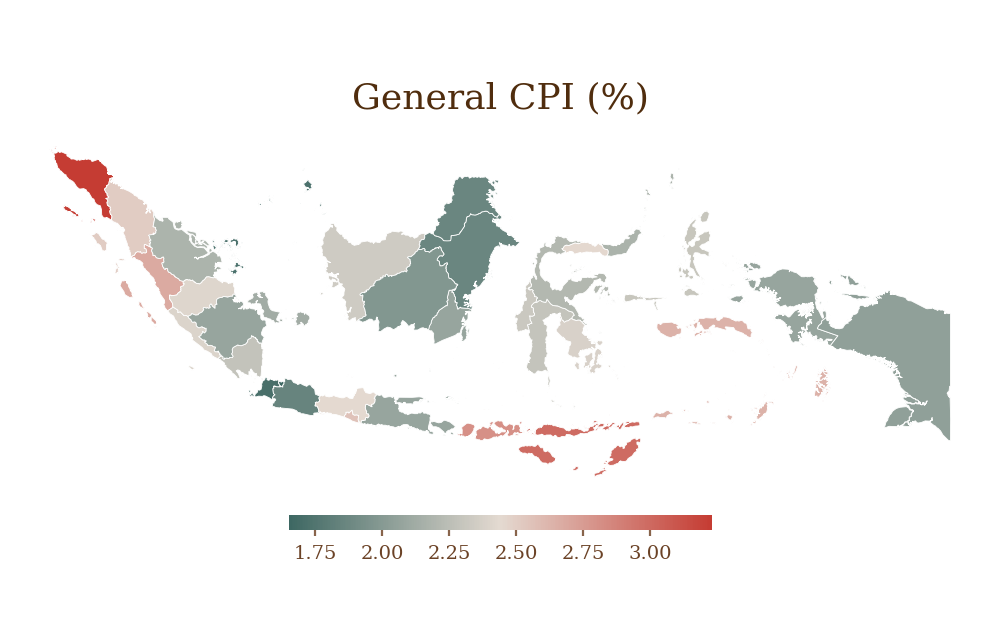
\includegraphics[width=0.69\linewidth]{map_S1_genCPI.png}
	\column{0.5\textwidth}\centering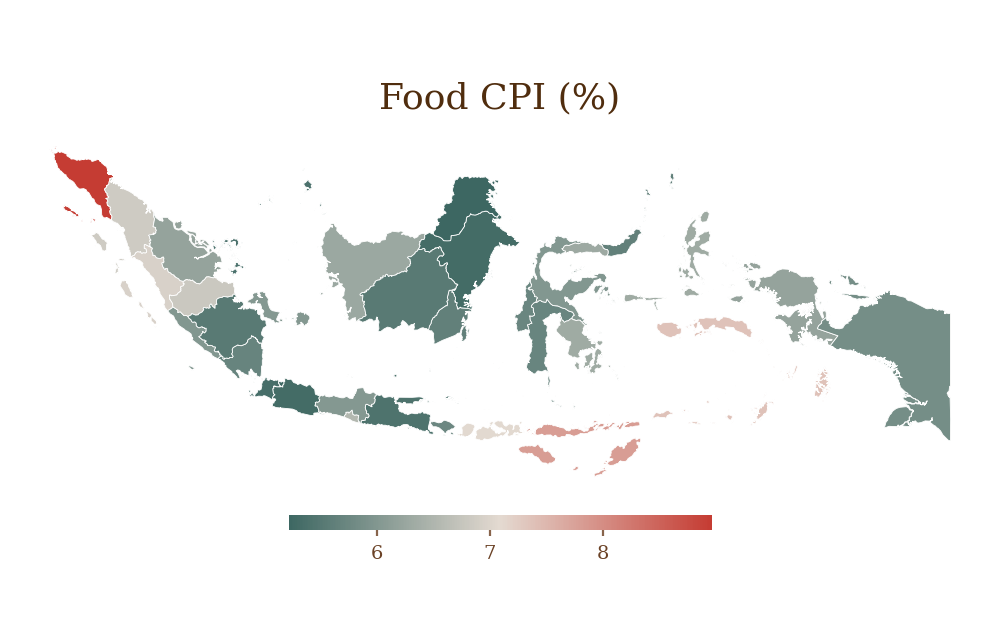
\includegraphics[width=0.69\linewidth]{map_S1_foodCPI.png}
\end{columns}
\vspace{-6pt}
\begin{columns}[T,onlytextwidth]
	\column{0.5\textwidth}\centering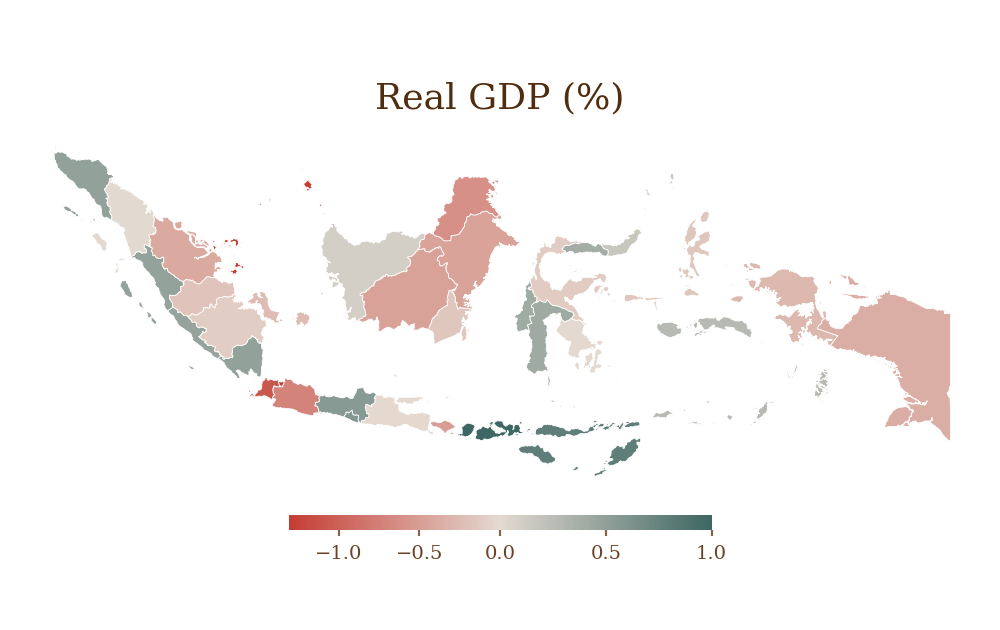
\includegraphics[width=0.69\linewidth]{map_S1_realGDP.png}
	\column{0.5\textwidth}\centering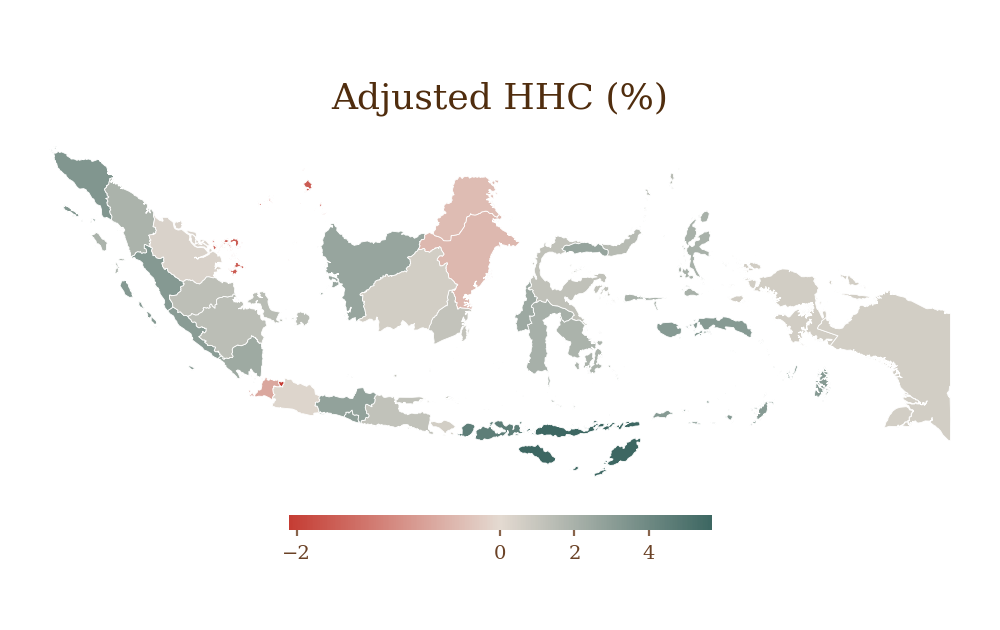
\includegraphics[width=0.69\linewidth]{map_S1_adjHHC.png}
\end{columns}
{\tiny\textcolor{lubrown}{\textbf{Highlights:}} NAD's large fruit demand shock drives the country's highest CPI ($3.23\%$), yet still nets $+3.37\%$. Only 5 provinces post net losses --- DKI, KepRi, Banten, KalTim, KalUt --- all combining modest local procurement with imported food inflation. NTT gains most ($+5.68\%$). \emph{Each map uses its own color scale.}}
\end{frame}

\begin{frame}{Provincial Impacts: Free Trade}
\centering
\begin{columns}[T,onlytextwidth]
	\column{0.5\textwidth}\centering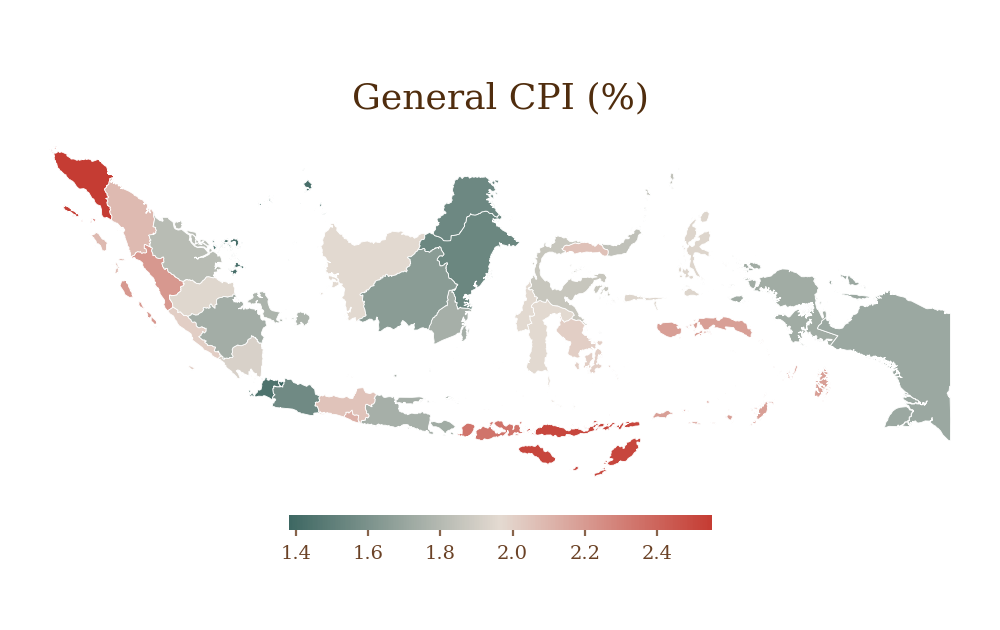
\includegraphics[width=0.69\linewidth]{map_S2_genCPI.png}
	\column{0.5\textwidth}\centering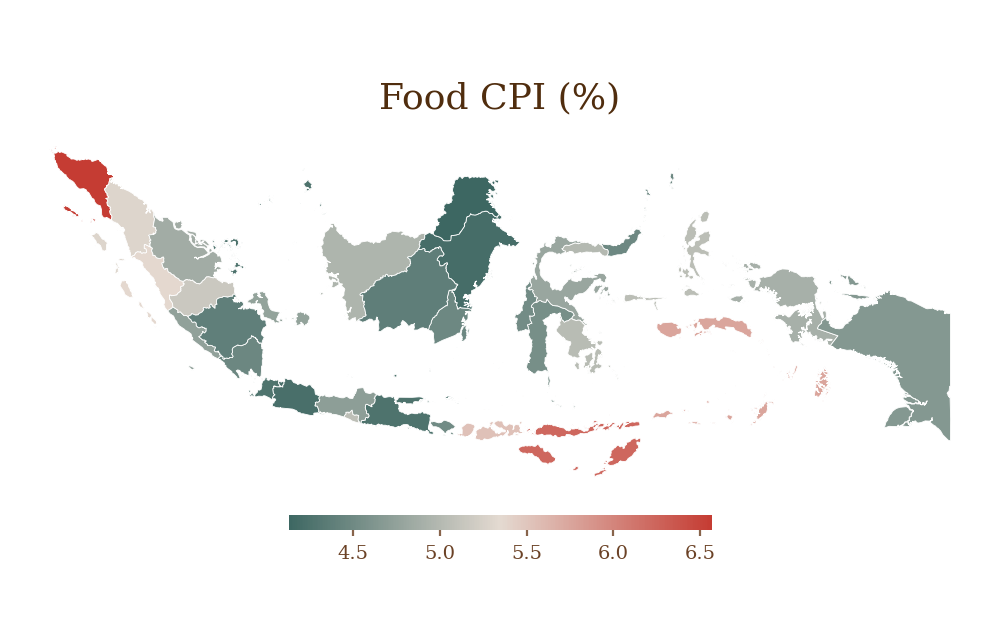
\includegraphics[width=0.69\linewidth]{map_S2_foodCPI.png}
\end{columns}
\vspace{-6pt}
\begin{columns}[T,onlytextwidth]
	\column{0.5\textwidth}\centering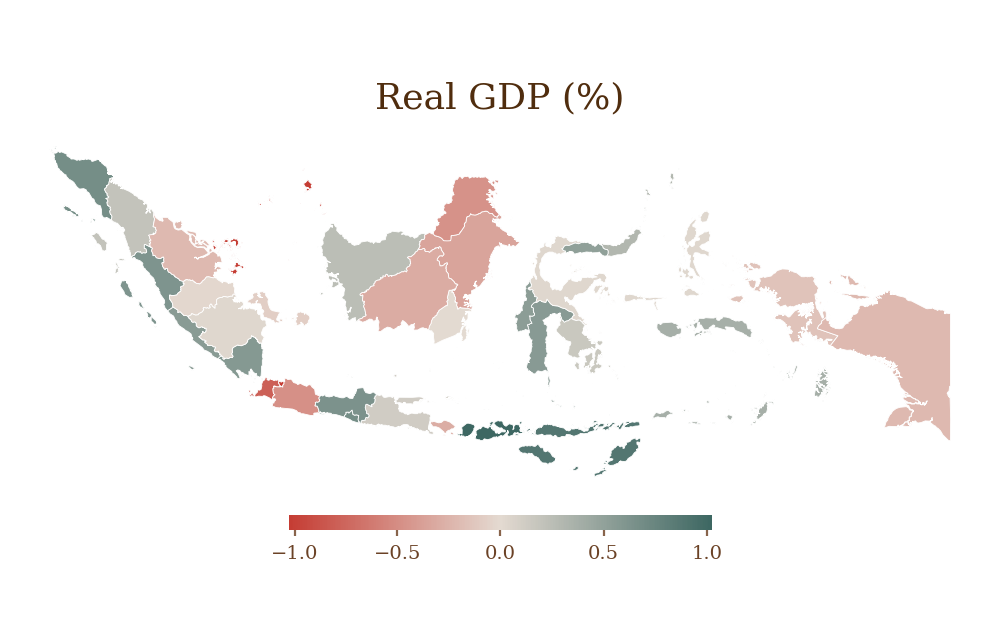
\includegraphics[width=0.69\linewidth]{map_S2_realGDP.png}
	\column{0.5\textwidth}\centering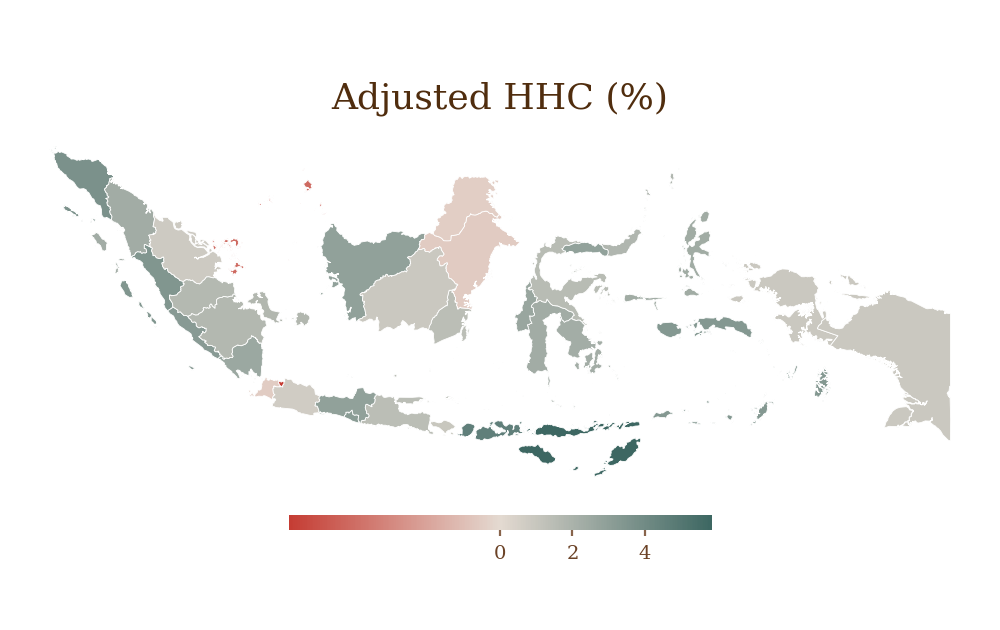
\includegraphics[width=0.69\linewidth]{map_S2_adjHHC.png}
\end{columns}
{\tiny\textcolor{lubrown}{\textbf{Highlights:}} Same 5 provinces remain net losers as under protection, but losses are smaller throughout (e.g.\ DKI improves to $-1.55\%$). Price increases ease nationwide relative to protection, and every province's welfare outcome improves. \emph{Each map uses its own color scale.}}
\end{frame}

\begin{frame}{Provincial Impacts: Productivity}
\centering
\begin{columns}[T,onlytextwidth]
	\column{0.5\textwidth}\centering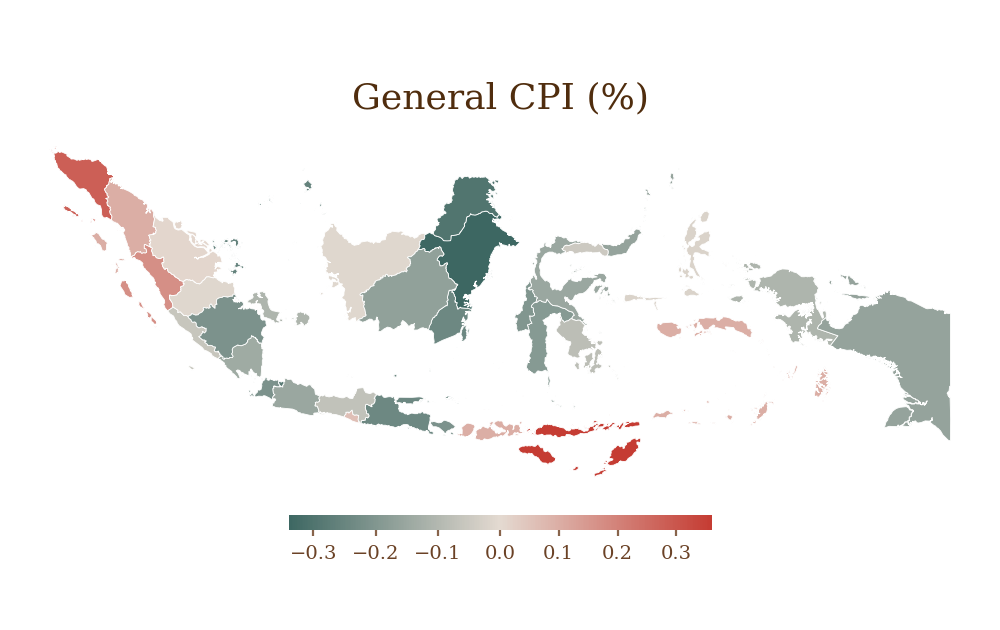
\includegraphics[width=0.69\linewidth]{map_S3_genCPI.png}
	\column{0.5\textwidth}\centering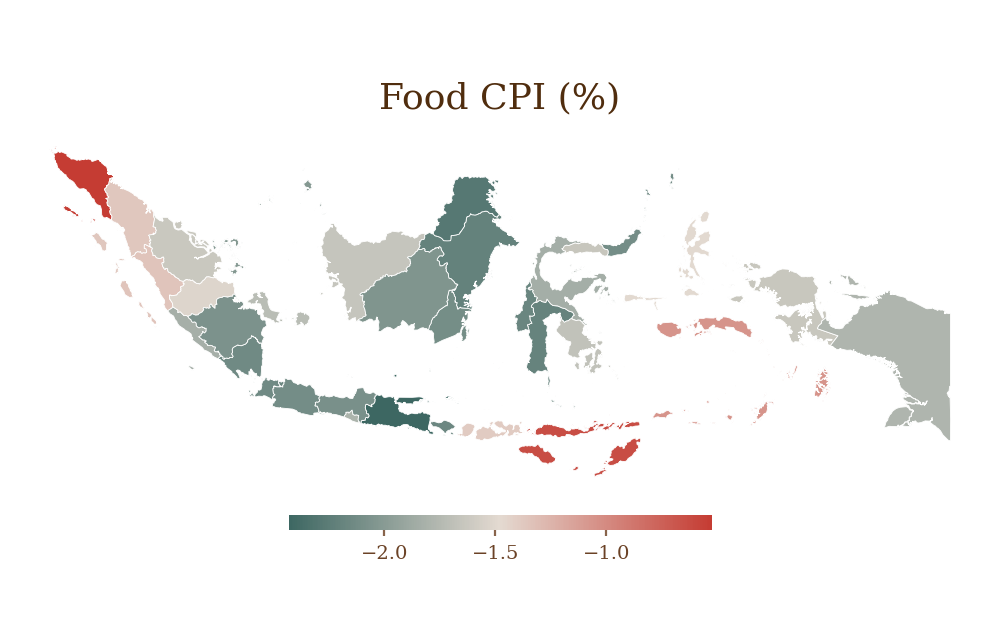
\includegraphics[width=0.69\linewidth]{map_S3_foodCPI.png}
\end{columns}
\vspace{-6pt}
\begin{columns}[T,onlytextwidth]
	\column{0.5\textwidth}\centering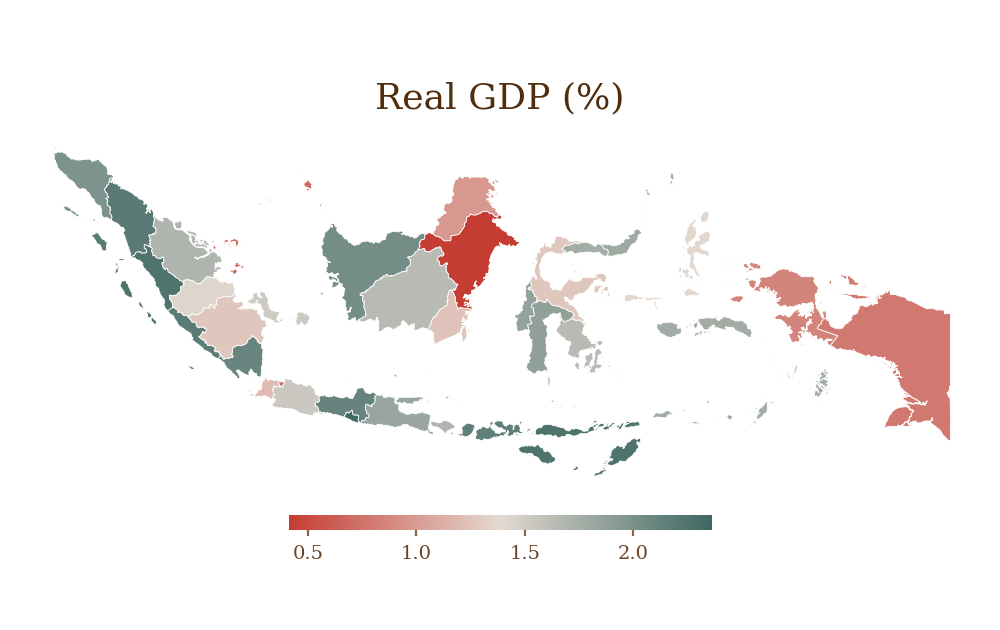
\includegraphics[width=0.69\linewidth]{map_S3_realGDP.png}
	\column{0.5\textwidth}\centering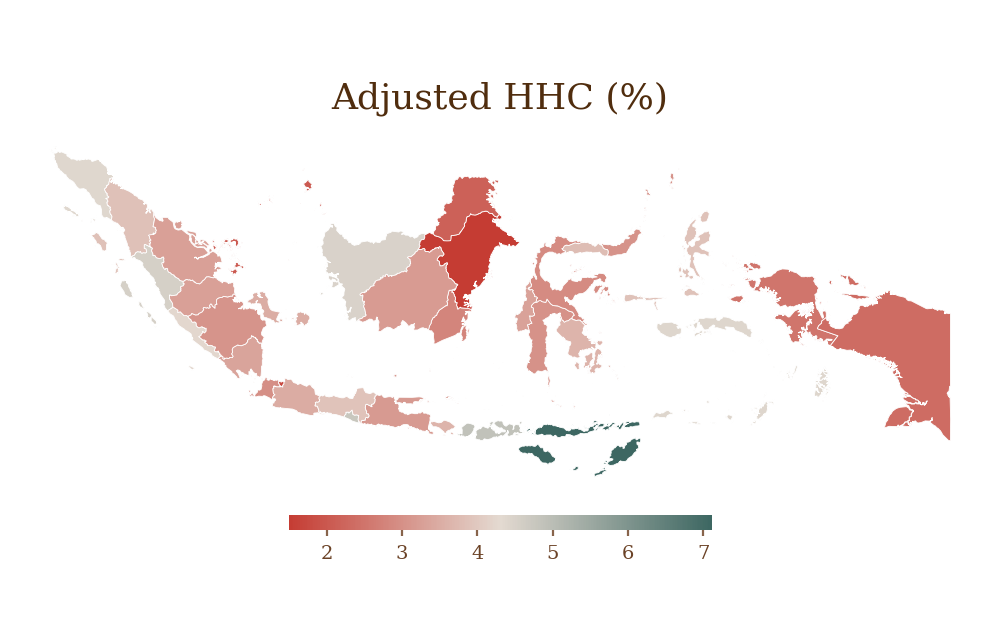
\includegraphics[width=0.69\linewidth]{map_S3_adjHHC.png}
\end{columns}
{\tiny\textcolor{lubrown}{\textbf{Highlights:}} All 34 provinces record positive adjusted welfare, ranging from $+1.49\%$ (KalTim) to $+7.11\%$ (NTT). General and food CPI turn negative almost everywhere --- MBG now makes food \emph{cheaper}, not more expensive. \emph{Each map uses its own color scale.}}
\end{frame}

\begin{frame}{Who Loses Under Protection --- and Why?}
\footnotesize
\begin{columns}[T,onlytextwidth]
	\column{0.35\textwidth}
	\textbf{5 of 34 provinces record net losses}
	\begin{itemize}\setlength\itemsep{5pt}
		\item DKI Jakarta: Adj.\ HHC $-2.08\%$ (CPI $+1.65\%$)
		\item Riau Islands (KepRi): $-1.67\%$ (CPI $+1.72\%$)
		\item Banten: $-0.68\%$ (CPI $+1.71\%$)
		\item East Kalimantan (KalTim): $-0.45\%$
		\item North Kalimantan (KalUt): $-0.39\%$
	\end{itemize}
	\column{0.65\textwidth}
	\textbf{Common structural feature}
	\begin{itemize}\setlength\itemsep{4pt}
		\item Modest local MBG procurement $\to$ small in-kind transfer.
		\item Yet exposed to food price inflation transmitted from producing provinces via inter-regional trade.
		\item Real GDP also contracts in all 5 (e.g.\ DKI $-1.30\%$, KepRi $-1.31\%$) --- non-food, urban/service economies left out of MBG's shift toward food production.
		\item DKI: fruit demand shock only 3.98\%, yet fruit prices rise 20.57\% --- driven by price transmission, not local demand.
		\item Contrast: NAD (highest CPI, 3.23\%) still nets $+3.37\%$; NTT nets the highest gain of any province, $+5.68\%$, from its outsized dairy procurement share.
	\end{itemize}
\end{columns}
\end{frame}

\begin{frame}{MBG's Progressive Geographic Incidence}
\centering
\begin{columns}[T,onlytextwidth]
	% Panel (a): Protection
	\begin{column}{0.32\textwidth}
		\centering\small\textbf{(a) Protection}
		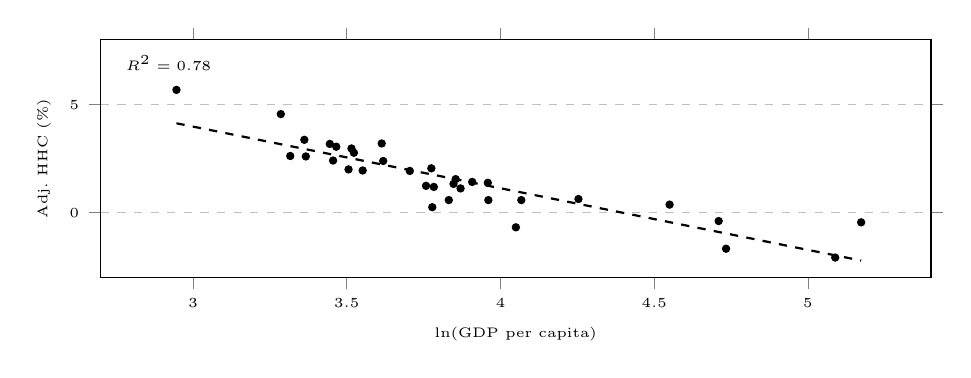
\begin{tikzpicture}
			\begin{axis}[
				width=\textwidth, height=4.6cm,
				xlabel={\tiny $\ln$(GDP per capita)},
				ylabel={\tiny Adj.\ HHC (\%)},
				xmin=2.7, xmax=5.4, ymin=-3, ymax=8,
				xtick={3,3.5,4,4.5,5},
				xticklabel style={font=\tiny}, yticklabel style={font=\tiny},
				xlabel style={font=\tiny}, ylabel style={font=\tiny},
				ymajorgrids=true, grid style=dashed, tick align=outside,
				]
				\addplot[only marks, mark=*, mark size=1.3pt, black]
				coordinates {(3.3621,3.37) (3.7052,1.93) (3.6138,3.20)
					(4.5500,0.37) (4.7337,-1.67) (3.8473,1.33) (3.9589,1.38)
					(3.9081,1.42) (3.4659,3.05) (3.6186,2.39) (5.0887,-2.08)
					(3.7782,0.25) (4.0501,-0.68) (3.5233,2.77) (3.5154,2.97)
					(3.7833,1.19) (3.3670,2.60) (3.9607,0.58) (3.8702,1.12)
					(5.1730,-0.45) (4.7096,-0.39) (3.8543,1.55) (3.3163,2.62)
					(3.7579,1.24) (3.7752,2.05) (3.4556,2.41) (3.5519,1.95)
					(3.8319,0.58) (3.2856,4.56) (2.9463,5.68) (3.4450,3.18)
					(3.5059,2.00) (4.2536,0.63) (4.0678,0.58)};
				\addplot[thick, black, dashed]
				coordinates {(2.9463,4.1345) (5.1730,-2.2184)};
				\node[anchor=north west, font=\tiny] at (axis cs:2.75,7.7) {$R^2=0.78$};
			\end{axis}
		\end{tikzpicture}
	\end{column}
	% Panel (b): Free Trade
	\begin{column}{0.32\textwidth}
		\centering\small\textbf{(b) Free Trade}
		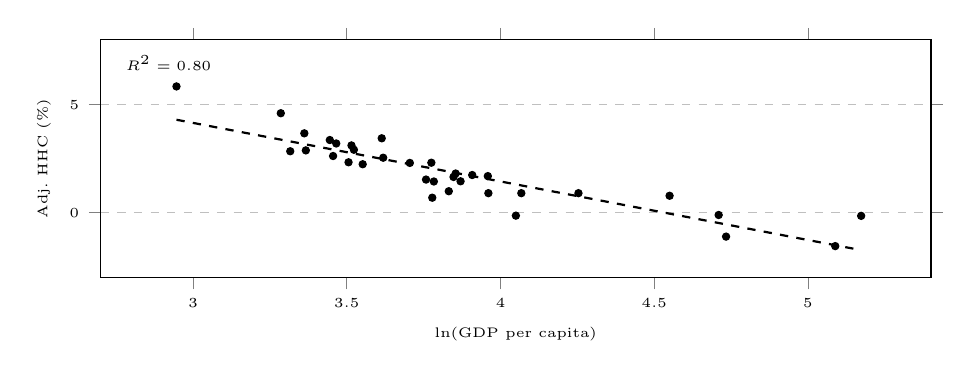
\begin{tikzpicture}
			\begin{axis}[
				width=\textwidth, height=4.6cm,
				xlabel={\tiny $\ln$(GDP per capita)},
				ylabel={\tiny Adj.\ HHC (\%)},
				xmin=2.7, xmax=5.4, ymin=-3, ymax=8,
				xtick={3,3.5,4,4.5,5},
				xticklabel style={font=\tiny}, yticklabel style={font=\tiny},
				xlabel style={font=\tiny}, ylabel style={font=\tiny},
				ymajorgrids=true, grid style=dashed, tick align=outside,
				]
				\addplot[only marks, mark=*, mark size=1.3pt, black]
				coordinates {(3.3621,3.67) (3.7052,2.30) (3.6138,3.44)
					(4.5500,0.78) (4.7337,-1.11) (3.8473,1.65) (3.9589,1.69)
					(3.9081,1.74) (3.4659,3.20) (3.6186,2.54) (5.0887,-1.55)
					(3.7782,0.69) (4.0501,-0.14) (3.5233,2.91) (3.5154,3.11)
					(3.7833,1.44) (3.3670,2.88) (3.9607,0.90) (3.8702,1.45)
					(5.1730,-0.15) (4.7096,-0.11) (3.8543,1.81) (3.3163,2.84)
					(3.7579,1.53) (3.7752,2.31) (3.4556,2.62) (3.5519,2.24)
					(3.8319,0.99) (3.2856,4.60) (2.9463,5.84) (3.4450,3.36)
					(3.5059,2.33) (4.2536,0.90) (4.0678,0.90)};
				\addplot[thick, black, dashed]
				coordinates {(2.9463,4.2981) (5.1730,-1.7362)};
				\node[anchor=north west, font=\tiny] at (axis cs:2.75,7.7) {$R^2=0.80$};
			\end{axis}
		\end{tikzpicture}
	\end{column}
	% Panel (c): Productivity
	\begin{column}{0.32\textwidth}
		\centering\small\textbf{(c) Productivity}
		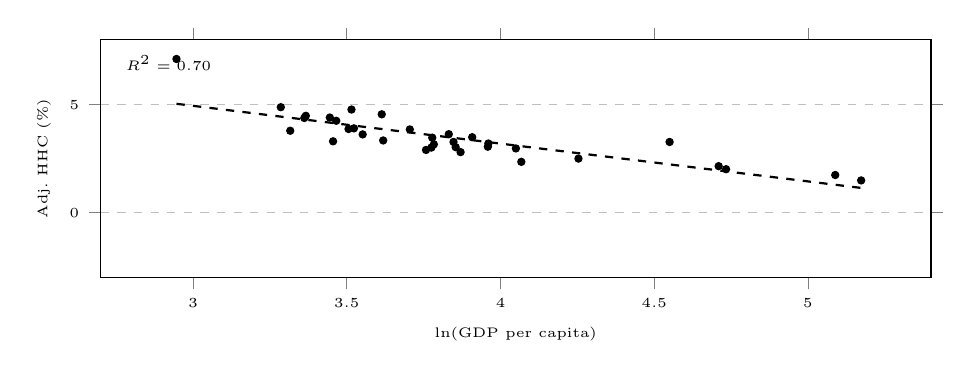
\begin{tikzpicture}
			\begin{axis}[
				width=\textwidth, height=4.6cm,
				xlabel={\tiny $\ln$(GDP per capita)},
				ylabel={\tiny Adj.\ HHC (\%)},
				xmin=2.7, xmax=5.4, ymin=-3, ymax=8,
				xtick={3,3.5,4,4.5,5},
				xticklabel style={font=\tiny}, yticklabel style={font=\tiny},
				xlabel style={font=\tiny}, ylabel style={font=\tiny},
				ymajorgrids=true, grid style=dashed, tick align=outside,
				]
				\addplot[only marks, mark=*, mark size=1.3pt, black]
				coordinates {(3.3621,4.38) (3.7052,3.85) (3.6138,4.55)
					(4.5500,3.27) (4.7337,2.01) (3.8473,3.27) (3.9589,3.05)
					(3.9081,3.49) (3.4659,4.25) (3.6186,3.34) (5.0887,1.74)
					(3.7782,3.47) (4.0501,2.97) (3.5233,3.90) (3.5154,4.77)
					(3.7833,3.16) (3.3670,4.48) (3.9607,3.20) (3.8702,2.80)
					(5.1730,1.49) (4.7096,2.15) (3.8543,3.03) (3.3163,3.79)
					(3.7579,2.90) (3.7752,3.01) (3.4556,3.30) (3.5519,3.62)
					(3.8319,3.63) (3.2856,4.88) (2.9463,7.11) (3.4450,4.40)
					(3.5059,3.87) (4.2536,2.50) (4.0678,2.35)};
				\addplot[thick, black, dashed]
				coordinates {(2.9463,5.0366) (5.1730,1.1423)};
				\node[anchor=north west, font=\tiny] at (axis cs:2.75,7.7) {$R^2=0.70$};
			\end{axis}
		\end{tikzpicture}
	\end{column}
\end{columns}
\smallskip
{\tiny\textcolor{gray}{Each panel plots adjusted household consumption (\% dev.\ from baseline) against $\ln$(provincial GDP per capita). Dashed line: OLS trend. Poorer provinces gain more, consistently across all three policy regimes.}}

\medskip
{\scriptsize\textcolor{lubrown}{\textbf{Key takeaway:}} The gradient is nearly identical under protection and free trade ($R^2=0.78, 0.80$) --- the progressive incidence is driven by MBG's procurement geography, not trade policy. Under productivity ($R^2=0.70$), even wealthier provinces gain substantially, narrowing the gap.}
\end{frame}

\section{Conclusion}

\begin{frame}{Key Findings}
\footnotesize
\begin{itemize}\setlength\itemsep{9pt}
	\item MBG is a demand-side macroeconomic event, not merely a nutritional transfer: welfare depends critically on the accompanying trade regime.
	\item \textbf{Protection}: general CPI $+2.08$pp, food CPI $+5.74$pp; broad inflation taxes away much of the transfer's real value; adjusted welfare still positive ($+0.79\%$) but 5 provinces are net losers.
	\item \textbf{Free Trade}: improves on protection (adjusted welfare $+1.13\%$; smaller provincial losses) but requires food imports to rise $12.61\%$ --- at odds with the self-sufficiency agenda.
	\item \textbf{Productivity}: all 34 provinces gain (adjusted welfare $+3.16\%$); food prices fall \emph{below} baseline; food imports remain essentially unchanged ($-0.05\%$).
	\item Progressive geographic incidence holds under all three regimes ($R^2=0.78$, $0.80$, $0.70$): poorer provinces consistently benefit more.
\end{itemize}
\end{frame}

\begin{frame}{Why Is MBG Progressive? Decomposing the Mechanism}
\footnotesize
\centering
\begin{tabular}{l r p{5.6cm}}
	\toprule
	\textbf{Indicator (Protection)} & \textbf{$r$ vs.\ $\ln$(GDPpc)} & \textbf{Reading} \\
	\midrule
	General CPI                    & $-0.77$ & Poorer provinces face slightly higher inflation \\
	Real GDP                       & $-0.79$ & Poorer provinces gain output share as production reallocates toward food \\
	Real HHC (no transfer)         & $-0.82$ & Combined price + output effect already favors poorer provinces \\
	Adjusted HHC (+ transfer)      & $-0.89$ & The transfer amplifies the progressivity further \\
	\bottomrule
\end{tabular}

\smallskip
\begin{itemize}\setlength\itemsep{3pt}
	\item[(a)] Poorer, less-connected provinces face \emph{modestly} higher inflation --- real, but a secondary effect.
	\item[(b)] Transfers are dramatically more valuable to poorer provinces: implied transfer value ranges from $+0.4$pp (DKI) to $+4.3$pp (NTT) of household consumption.
	\item[(c)] Richer provinces don't pay an \emph{inflation} tax --- they pay an \textbf{output-reallocation tax}: MBG shifts economic activity toward food-producing, mostly poorer provinces, contracting real GDP in richer, non-food, urban economies.
\end{itemize}

{\scriptsize\textcolor{lubrown}{\textbf{Net:}} (a)+(c) on the cost side are outweighed by (b) on the benefit side --- progressivity is driven by \emph{who produces the food and receives the transfer}, not by who pays more at the register.}
\end{frame}

\begin{frame}{Policy Implications}
\footnotesize
\begin{itemize}\setlength\itemsep{9pt}
	\item The welfare impact of MBG depends as much on the \emph{policy environment} as on the program design itself.
	\item Free trade is an immediately available, no-cost improvement --- but politically incompatible with Indonesia's entrenched self-sufficiency narrative.
	\item Productivity delivers the best outcome on both welfare \emph{and} self-sufficiency grounds, but feasibility varies by sector: required TFP gains range from $0.75\%$ (bread \& biscuit) to $10.00\%$ (fruits) --- most within Indonesia's historical productivity performance, fruits the exception.
	\item \textbf{Realistic near-term mix}: trade liberalisation for import-responsive sectors + targeted productivity investment (dairy, poultry, abattoir) where TFP requirements are attainable.
	\item The central question is not \emph{whether} to pursue food self-sufficiency alongside MBG, but \emph{through which instruments} --- and at what pace.
\end{itemize}
\end{frame}

\begin{frame}[c]
\centering
{\Large\textcolor{lubrown}{\textbf{Feeding a Nation}}}\\[10pt]
{\large\textit{Thank you for listening!\\[4pt] Questions and comments welcome.}}
\end{frame}

\end{document}
